\documentclass[../../book.tex]{subfiles}
\begin{document}
\graphicspath{{./}}
\chaptertitle{Steady-State Error Analysis}{6}

% ===========================================================================
\section{Introduction}
\label{sec:intro}
% ===========================================================================

The PID article established how a feedback controller shapes the \emph{transient}
response --- settling time, overshoot, damping ratio.  But there is a second
performance dimension that transient analysis says nothing about: what happens
\emph{after} the transients die out?  If a vessel is commanded to hold 5\,m/s,
does it actually reach 5\,m/s, or does it settle 0.3\,m/s short?  If it is
commanded to track a linearly increasing waypoint sequence, does the position
error grow without bound, or does it converge to a fixed lag (constant offset)?

\emph{Steady-state error} is the difference between the desired output and the
actual output after transients have decayed.  It is the next essential tool for
describing and specifying the performance of a feedback system.


In this article we derive steady-state error expressions for
\emph{unity negative feedback} systems (\cref{fig:unity_fb}) with \emph{stable}
closed-loop dynamics.  The final value theorem, on which all steady state error analysis rests, is only valid
for stable systems. 

% ===========================================================================
\section{Deriving the General Error Formula}
\label{sec:derivation}
% ===========================================================================

\begin{figure}[htbp]
\centering
\begin{tikzpicture}[
  >=Latex, thick,
  block/.style = {draw, rectangle, minimum height=2.5em, minimum width=4.5em},
  sum/.style   = {draw, circle, inner sep=0pt, minimum size=1.2em},
]
  \node[coordinate]                   (rin)  {};
  \node[sum,   right=1.6cm of rin]    (sum)  {};
  \node[block, right=2.4cm of sum]    (G)    {$G(s)$};
  \node[coordinate, right=1.6cm of G] (yout) {};

  \node[font=\scriptsize, inner sep=0pt, anchor=south east] at (sum.north west) {$+$};
  \node[font=\scriptsize, inner sep=0pt, anchor=north east] at (sum.south west) {$-$};

  \draw[->] (rin)  -- node[above]{$R(s)$}  (sum);
  \draw[->] (sum)  -- node[above]{$E(s)$}  (G);
  \draw[->] (G)    -- node[above]{$Y(s)$}  (yout);

  \coordinate (fbk) at ($(G.east)!0.5!(yout)$);
  \draw[->] (fbk) -- ++(0,-1.6) -| (sum.south);
\end{tikzpicture}
\caption{Unity-feedback loop.  $G(s)$ is the open-loop forward transfer function
  (plant $\times$ controller combined).  The error signal is $E(s) = R(s) - Y(s)$.}
\label{fig:unity_fb}
\end{figure}

For the loop in \cref{fig:unity_fb}, the plant output is $Y(s) = G(s)E(s)$.
Substituting into the error definition $E(s) = R(s) - Y(s)$:
\[
  E(s) = R(s) - G(s)E(s)
  \implies
  E(s) = \frac{R(s)}{1 + G(s)}
\]

We want the long-run value of $e(t)$.  The \textbf{final value theorem} avoids
a full inverse Laplace transform:
\[
  e(\infty) = \lim_{t \to \infty} e(t) = \lim_{s \to 0} s\,E(s)
\]
This is valid as long as $sE(s)$ has no poles on or to the right of the
imaginary axis --- which holds whenever the closed-loop system is stable.
Substituting:

\begin{equation}
  \boxed{e(\infty) = \lim_{s \to 0} \frac{s\,R(s)}{1 + G(s)}}
  \label{eq:ess_general}
\end{equation}

\textbf{This is the master equation.}  Everything that follows is obtained by
substituting specific inputs $R(s)$ and specific open-loop transfer functions
$G(s)$.  No new derivation is needed; only the evaluation of limits.

\textbf{Notation.}  Throughout this article, $G(s) = C(s)\,P(s)$ denotes the
\emph{combined} open-loop forward transfer function --- controller times plant.
This is \emph{overloaded notation}: the symbol $G(s)$ sometimes refers to the
plant alone, sometimes to the controller, and sometimes to their product,
depending on context.  In steady-state error analysis the convention is always
$G(s) = C(s)\,P(s)$: the full forward path from the error signal to the plant
output.  The formula depends only on that product, not on how it is divided
between $C(s)$ and $P(s)$.

% ===========================================================================
\section{Test Inputs: Step, Ramp, Parabola}
\label{sec:inputs}
% ===========================================================================

The choice of test input depends on what the controlled system must track.  We typically test with three standard inputs, which can be thought of as three different scenarios:
\begin{itemize}
  \item \textbf{Step.}  A step reference represents a sudden change in desired position or speed that must then be held.  A vessel commanded to a new waypoint and then to hold position faces a step problem.

  \item \textbf{Ramp.}  A ramp reference represents a target moving at constant velocity.  The tracking system must continuously follow a linearly increasing reference.

  \item \textbf{Parabola.}  A parabola reference represents a target with constant acceleration.  The reference grows quadratically, which is the hardest case to follow.
\end{itemize}

\begin{table}[htbp]
\centering
\caption{Standard test inputs for steady-state error analysis.}
\label{tab:inputs}
\begin{tabular}{llcc}
\toprule
Name     & Physical interpretation & $r(t)$             & $R(s)$   \\
\midrule
Step     & Constant position       & $1$                & $1/s$    \\
Ramp     & Constant velocity       & $t$                & $1/s^2$  \\
Parabola & Constant acceleration   & $\frac{1}{2}t^2$   & $1/s^3$  \\
\bottomrule
\end{tabular}
\end{table}

\subsection{Defense Analogies}

These three test inputs map  onto the three targeting
scenarios that appear in fire control and weapon-system tracking:

\textbf{Stationary target.}  A fixed location, a satellite in geostationary
orbit, a ship at anchor --- the tracking system only needs to acquire and hold a
fixed pointing angle.  The test input is a step.  Even a small persistent pointing
bias (nonzero step error) causes a miss.

\textbf{Constant-velocity target.}  A surface ship at steady speed, a satellite
in circular orbit, an aircraft in level flight.  The system must continuously
\emph{follow} a moving position.  A Close-In Weapon System (CIWS) director
computing gun lead angles, or a satellite dish tracking a low-earth-orbit pass,
faces exactly this problem.  The ramp tracking error is the steady-state angular
or positional lag behind the target.

\textbf{Maneuvering (accelerating) target.}  A ballistic missile under thrust,
an aircraft in a turn, a UAV executing an evasive break.  The target's
velocity itself is changing.  Even a system that tracks constant-velocity targets
perfectly will accumulate growing error against an accelerating target unless the
control system has sufficient integration in its forward path.  This is the
parabolic case.

The sophistication required of the feedback system increases across the three
cases.  As we will see, each successive case demands one additional integrator
in the open-loop forward path to maintain bounded error.

This progression captures a tension that runs through all of control engineering:
improving steady-state accuracy generally costs something --- slower transient
response, reduced stability margin, or both.  Knowing which side of that
tradeoff you are on is as important as knowing the formula.

% ===========================================================================
\section{Step, Ramp, and Parabola Errors from \cref{eq:ess_general}}
\label{sec:three_cases}
% ===========================================================================

\subsection{Step Input}

With $R(s) = 1/s$, \cref{eq:ess_general} gives:
\begin{equation}
  e_{\rm step}(\infty)
    = \lim_{s \to 0} \frac{s \cdot (1/s)}{1 + G(s)}
    = \lim_{s \to 0} \frac{1}{1 + G(s)}
    = \frac{1}{1 + \lim_{s\to 0} G(s)}
  \label{eq:ess_step}
\end{equation}

The key quantity is $\lim_{s\to 0} G(s)$, the DC gain of the open-loop
transfer function.
\begin{itemize}
  \item If $G(s)$ has \emph{no poles at $s = 0$}: the DC gain is a finite
    constant, and the step error is nonzero.
  \item If $G(s)$ has \emph{one or more poles at $s = 0$} (integrators):
    $G(0) = \infty$, and $e_{\rm step} = 0$.
\end{itemize}

This is exactly what we found in the PID article: a proportional-only controller
leaves a residual step error, while adding an integrator (PI or I action) drives
it to zero.

\subsection{Ramp Input}

With $R(s) = 1/s^2$:
\begin{equation}
  e_{\rm ramp}(\infty)
    = \lim_{s \to 0} \frac{s \cdot (1/s^2)}{1 + G(s)}
    = \lim_{s \to 0} \frac{1}{s\bigl(1 + G(s)\bigr)}
    = \frac{1}{\lim_{s \to 0}\, s\,G(s)}
  \label{eq:ess_ramp}
\end{equation}

The key quantity is now $\lim_{s\to 0} s\,G(s)$.  As $s \to 0$, the added
factor of $s$ cancels one pole at the origin:
\begin{itemize}
  \item \emph{No integrators in $G(s)$}: $\lim s\,G(s) = 0$, so
    $e_{\rm ramp} = \infty$.  The output falls infinitely far behind a ramp
    input.
  \item \emph{One integrator}: write $G(s) = \widetilde{G}(s)/s$, where
    $\widetilde{G}(s)$ is $G(s)$ with the single integrator removed, so
    $\widetilde{G}(0)$ is finite and nonzero.  Then $\lim s\,G(s) =
    \widetilde{G}(0)$ and $e_{\rm ramp}$ is finite.
  \item \emph{Two or more integrators}: $\lim s\,G(s) = \infty$, so
    $e_{\rm ramp} = 0$.
\end{itemize}

\subsection{Parabola Input}

With $R(s) = 1/s^3$:
\begin{equation}
  e_{\rm para}(\infty)
    = \lim_{s \to 0} \frac{s \cdot (1/s^3)}{1 + G(s)}
    = \frac{1}{\lim_{s \to 0}\, s^2\,G(s)}
  \label{eq:ess_para}
\end{equation}

\begin{itemize}
  \item \emph{Zero or one integrators}: $\lim s^2\,G(s) = 0 \Rightarrow
    e_{\rm para} = \infty$.
  \item \emph{Two integrators}: $\lim s^2\,G(s)$ is finite and nonzero
    $\Rightarrow$ finite parabola error.
  \item \emph{Three or more integrators}: $\lim s^2\,G(s) = \infty \Rightarrow
    e_{\rm para} = 0$.
\end{itemize}

The pattern is clear: each successive input type requires one more integrator in
$G(s)$ to achieve finite (or zero) error.

% ===========================================================================
\section{System Type}
\label{sec:system_type}
% ===========================================================================

The behavior above depends on how many poles $G(s)$ has at the
origin.  The number of poles at $s = 0$ (the origin) is the \emph{system type}.

\textbf{Definition.}  The \emph{system type} is the number $n$ of pure
integrators in the open-loop forward transfer function:
\begin{equation}
  G(s) = \frac{K\,(s + z_1)(s + z_2)\cdots}{s^n(s + p_1)(s + p_2)\cdots}
  \label{eq:G_form}
\end{equation}
A system is \emph{Type 0} when $n = 0$, \emph{Type 1} when $n = 1$,
\emph{Type 2} when $n = 2$, and so on.

System type is a property of the \emph{combined} open-loop transfer function ---
controller times plant, $G(s) = C(s)\,P(s)$ (\cref{fig:cl_with_type}).  Adding
an integrator to the controller (e.g., converting P to PI) increments the type
by one.

\begin{figure}[htbp]
\centering
\begin{tikzpicture}[
  >=Latex, thick,
  block/.style = {draw, rectangle, minimum height=2.5em, minimum width=4.5em},
  sum/.style   = {draw, circle, inner sep=0pt, minimum size=1.2em},
]
  \node[coordinate]                   (rin)  {};
  \node[sum,   right=1.6cm of rin]    (sum)  {};
  \node[block, right=2.0cm of sum]    (C)    {$C(s)$};
  \node[block, right=1.6cm of C]      (P)    {$P(s)$};
  \node[coordinate, right=1.6cm of P] (yout) {};

  \node[font=\scriptsize, inner sep=0pt, anchor=south east] at (sum.north west) {$+$};
  \node[font=\scriptsize, inner sep=0pt, anchor=north east] at (sum.south west) {$-$};

  \draw[->] (rin)  -- node[above]{$R(s)$} (sum);
  \draw[->] (sum)  -- node[above]{$E(s)$} (C);
  \draw[->] (C)    -- node[above]{$U(s)$} (P);
  \draw[->] (P)    -- node[above]{$Y(s)$} (yout);

  \coordinate (fbk) at ($(P.east)!0.5!(yout)$);
  \draw[->] (fbk) -- ++(0,-1.6) -| (sum.south);

  \node[draw, dashed, inner sep=8pt, fit=(C)(P),
        label=above:{$G(s) = C(s)\,P(s)$}] {};
\end{tikzpicture}
\caption{Unity-feedback loop showing controller $C(s)$ and plant $P(s)$
  separately.  The dashed box is the open-loop forward transfer function
  $G(s) = C(s)\,P(s)$.  System type is a property of $G(s)$ --- the combined
  product, regardless of how poles are distributed between $C$ and $P$.}
\label{fig:cl_with_type}
\end{figure}

The three limits from \cref{sec:three_cases} now read directly from the type:

\begin{center}
\begin{tabular}{lccc}
\toprule
 & $\lim_{s\to 0} G(s)$ & $\lim_{s\to 0} s\,G(s)$ & $\lim_{s\to 0} s^2\,G(s)$ \\
\midrule
Type 0 & $K$ (finite) & $0$          & $0$          \\
Type 1 & $\infty$     & $K_v$ (finite) & $0$          \\
Type 2 & $\infty$     & $\infty$     & $K_a$ (finite) \\
\bottomrule
\end{tabular}
\end{center}

Higher type is not always better.  Each additional integrator makes the loop
harder to stabilize and more sensitive to noise and model error.  Type~0 is
the most common; Type~1 is used when ramp tracking is required; Type~2 is
uncommon and requires careful compensator design to maintain stability.

\textbf{Example.}  Consider the first-order plant $P(s) = 5/(s+5)$ (Type~0).
The table shows what happens as the controller changes:

\begin{center}
\begin{tabular}{llcc}
\toprule
Controller $C(s)$ & Open-loop $G(s) = C(s)P(s)$ & Type & Step error \\
\midrule
$K_P = 2$ (P only) & $\dfrac{10}{s+5}$                 & 0 & $\dfrac{1}{1+2} = \tfrac{1}{3}$ \\[9pt]
$K_P + K_I/s$ (PI) & $\dfrac{5(K_P s + K_I)}{s(s+5)}$ & 1 & $0$ \\[9pt]
\bottomrule
\end{tabular}
\end{center}

The plant is identical in both rows.  Adding $K_I/s$ to the controller increments
$G(s)$ from Type~0 to Type~1 and drives the step error to zero.

% ===========================================================================
\section{Static Error Constants}
\label{sec:error_constants}
% ===========================================================================

The three limits that appear in \cref{eq:ess_step,eq:ess_ramp,eq:ess_para} are
given names because they appear so frequently:

\begin{align}
  K_x &= \lim_{s \to 0} G(s)         \label{eq:Kx} \\[4pt]
  K_v &= \lim_{s \to 0} s\,G(s)      \label{eq:Kv} \\[4pt]
  K_a &= \lim_{s \to 0} s^2\,G(s)    \label{eq:Ka}
\end{align}

These are the \emph{static error constants} (position, velocity, and
acceleration constants, respectively).

(Many textbooks write the position constant as $K_p$.  We
use $K_x$ throughout to avoid confusion with the proportional gain $K_P$
of a PID controller, which appears in the same design calculations.)

With this shorthand, the errors become:
\begin{align}
  e_{\rm step}(\infty) &= \frac{1}{1 + K_x} \label{eq:ess_Kx} \\[4pt]
  e_{\rm ramp}(\infty) &= \frac{1}{K_v}     \label{eq:ess_Kv} \\[4pt]
  e_{\rm para}(\infty) &= \frac{1}{K_a}     \label{eq:ess_Ka}
\end{align}

These are identical to \cref{eq:ess_step,eq:ess_ramp,eq:ess_para} ---
the constants are simply names for the limits already evaluated.

\subsection{Steady State Error Specification}

A single error constant encodes system type, test input, and error magnitude
simultaneously.  Given the specification $K_v = 20$, you can immediately
conclude:
\begin{enumerate}
  \item The system is \emph{stable} (otherwise the spec is undefined).
  \item The system is \emph{Type 1} --- only Type 1 has a finite nonzero $K_v$
    (Type 0 gives $K_v = 0$; Type 2 gives $K_v = \infty$).
  \item The relevant test input is a \emph{ramp}.
  \item The steady-state ramp error per unit slope is $1/K_v = 0.05 = 5\%$.
\end{enumerate}

\subsection{The Summary Table Falls Out of One Formula}

\Cref{tab:sse_summary} collects every case.  Every entry follows directly from
\cref{eq:ess_general} --- no new derivations or memorization required.  The
diagonal pattern is the key: Type $n$ achieves zero error for the step and all
simpler inputs, finite error for input type $n$ (the one that matches the
number of integrators), and infinite error for harder inputs.

\begin{table}[htbp]
\centering
\caption{Steady-state errors as a function of system type and input.  Every
  entry follows from \cref{eq:ess_general}.  $\infty$ indicates the output
  diverges from the reference.}
\label{tab:sse_summary}
\begin{tabular}{lccc}
\toprule
 & \multicolumn{3}{c}{System Type} \\
\cmidrule(lr){2-4}
Input    & Type 0              & Type 1              & Type 2 \\
\midrule
Step     & $\dfrac{1}{1+K_x}$ & $0$                 & $0$    \\[10pt]
Ramp     & $\infty$            & $\dfrac{1}{K_v}$   & $0$    \\[10pt]
Parabola & $\infty$            & $\infty$            & $\dfrac{1}{K_a}$ \\[10pt]
\bottomrule
\end{tabular}
\end{table}

\begin{figure}[htbp]
\centering
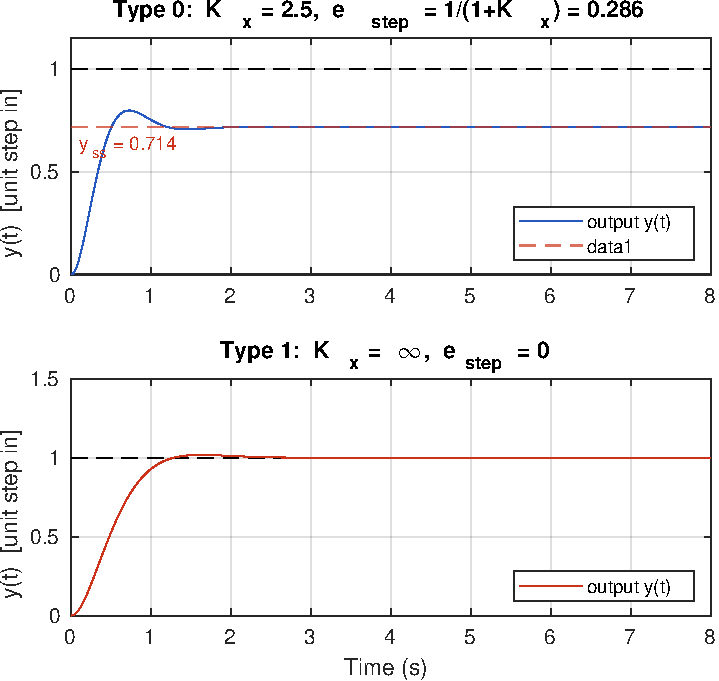
\includegraphics[width=0.75\linewidth]{images/sse_step_compare.pdf}
\caption{Step response comparison.  \emph{Top:} Type 0 system
  ($G_0 = 20/\bigl((s+2)(s+4)\bigr)$, $K_x = 2.5$) settles with a finite
  error below the reference.  \emph{Bottom:} Type 1 system
  ($G_1 = 10/\bigl(s(s+5)\bigr)$) tracks the step exactly.}
\label{fig:step_compare}
\end{figure}

\begin{figure}[htbp]
\centering
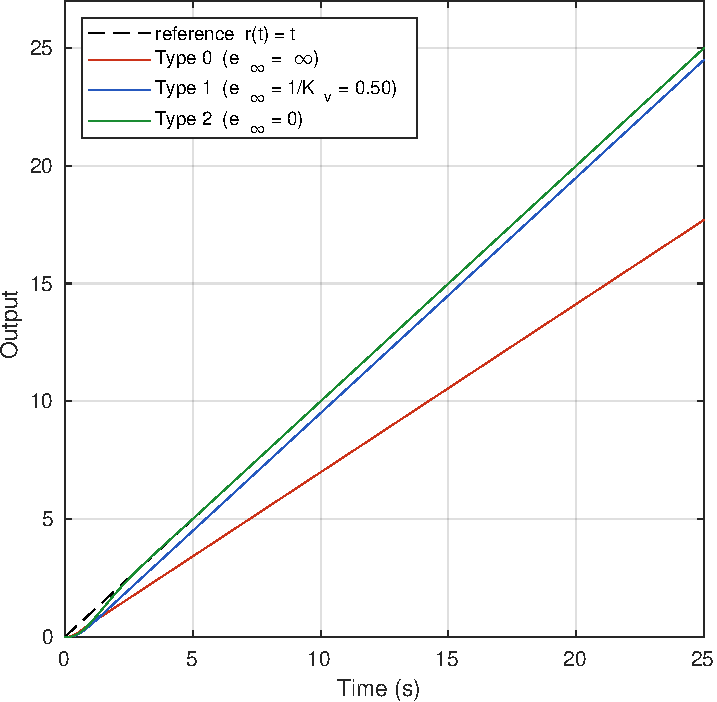
\includegraphics[width=0.675\linewidth]{images/sse_ramp_compare.pdf}
\caption{Ramp responses for three system types, all with unity feedback.
  Type 0 diverges (output increasingly lags behind).
  Type 1 converges to a constant lag of $1/K_v$.
  Type 2 converges to the ramp with zero steady-state error.}
\label{fig:ramp_compare}
\end{figure}

% ===========================================================================
\section{Design: Choosing Gain to Meet an Error Specification}
\label{sec:design}
% ===========================================================================

In many cases the system type is set by the physics and controller architecture,
leaving a scalar forward gain $K$ as the adjustable parameter.  An error
specification translates directly into a requirement on $K$.

\subsection{Procedure}

\begin{enumerate}
  \item Identify the system type from $G(s)$.
  \item Write the relevant error constant ($K_x$, $K_v$, or $K_a$) in terms
    of $K$ by evaluating the limit.
  \item Solve for the $K$ that satisfies the error requirement.
\end{enumerate}

\subsection{Example}

\textbf{Problem.} The open-loop transfer function of a position control system is:
\[
  G(s) = \frac{K(s + 3)}{s(s + 6)(s + 10)}
\]
Find $K$ such that the steady-state ramp error is 5\,\%.

\medskip
\textit{Step 1: System type.} One factor of $s$ in the denominator $\Rightarrow$
Type 1.  Ramp tracking yields a finite error.

\medskip
\textit{Step 2: Velocity constant.}
\[
  K_v = \lim_{s \to 0} s\,G(s)
      = \lim_{s \to 0} \frac{K\,s(s+3)}{s(s+6)(s+10)}
      = \frac{3K}{60}
      = \frac{K}{20}
\]

\textit{Step 3: Solve for $K$.} A 5\,\% ramp error requires $e_{\rm ramp} = 1/K_v = 0.05$, so $K_v = 20$:
\[
  \frac{K}{20} = 20 \implies \boxed{K = 400}
\]

\begin{figure}[htbp]
\centering
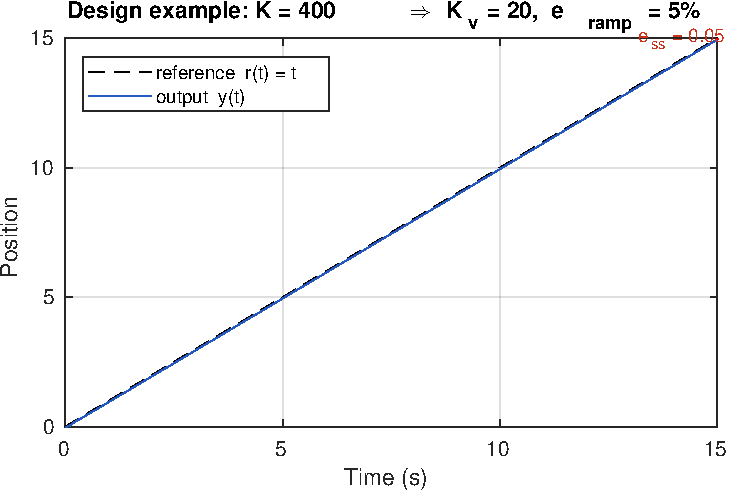
\includegraphics[width=0.64\linewidth]{images/sse_design.pdf}
\caption{Ramp response for the design example ($K = 400$).  After transients
  settle, the output runs parallel to the reference with a constant offset of
  0.05, confirming the $e_{\rm ramp} = 5\,\%$ specification for a unit-slope ramp.}
\label{fig:design}
\end{figure}

% ===========================================================================
\section{Eliminating Steady-State Error with an Integrator}
\label{sec:integrator}
% ===========================================================================

Adding integral action to the controller is the canonical way to eliminate
steady-state error.  The system type analysis in \cref{sec:system_type}
tells us \emph{that} it works (the type goes up by one); this section
explains \emph{why} it works at a physical level.

\subsection{The Adaptation Argument}

The integrator contribution to the control signal is:
\[
  u_I(t) = K_I \int_0^t e(\tau)\,d\tau
\]
What must be true at steady state in a \emph{stable} closed loop?

\begin{itemize}
  \item At steady state every signal is constant: $\dot y = 0$, $\dot e = 0$,
    $\dot u = 0$.
  \item The derivative of the integrator output is $\dot u_I = K_I\, e(t)$.
  \item For $u_I$ to be constant at steady state, $\dot u_I = 0$, which
    requires $e(t) = 0$.
\end{itemize}


Integration enables the controller to \emph{adapt} to persistent errors.  If the output is at all below the
setpoint, $e > 0$, the integrator output grows, along with the input to the plant.
It stops growing only when $e = 0$ --- regardless of unmodeled drag, fuel
consumption changing the vehicle's mass, wind, or current opposing the vessel.
The integrator compensates automatically for any source of steady-state offset.


\subsection{Effect on System Type}

\Cref{fig:pi_structure} shows the PI controller structure.  The error $E(s)$
drives both paths: the proportional path $K_P E(s)$ provides immediate response,
and the integrator path $K_I E(s)/s$ provides the accumulated bias.
Combining, the open-loop transfer function becomes:
\[
  G(s) = \underbrace{\frac{K_P s + K_I}{s}}_{C(s)}\cdot P(s)
\]
The factor of $s$ in the denominator is the integrator --- it increments the
system type by one relative to $K_P\cdot P(s)$ alone.

\begin{figure}[htbp]
\centering
\begin{tikzpicture}[
  >=Latex, thick,
  block/.style = {draw, rectangle, minimum height=2.5em, minimum width=5em},
  sum/.style   = {draw, circle, inner sep=0pt, minimum size=1.2em},
]
  \node[coordinate]                    (rin)  {};
  \node[sum,   right=1.4cm of rin]     (sum)  {};
  \node[block, right=1.8cm of sum]     (Kp)   {$K_P$};
  \node[sum,   right=1.8cm of Kp]      (usum) {};
  \node[block, right=1.8cm of usum]    (P)    {$P(s)$};
  \node[coordinate, right=1.4cm of P]  (yout) {};

  \node[block, below=1.0cm of Kp]      (Int)  {$K_I/s$};

  \node[font=\scriptsize, inner sep=0pt, anchor=south east] at (sum.north west)  {$+$};
  \node[font=\scriptsize, inner sep=0pt, anchor=north east] at (sum.south west)  {$-$};
  \node[font=\scriptsize, inner sep=0pt, anchor=north east] at (usum.south west) {$+$};
  \node[font=\scriptsize, inner sep=0pt, anchor=south east] at (usum.north west) {$+$};

  \draw[->] (rin)  -- node[above]{$R(s)$} (sum);
  \draw[->] (sum)  -- node[above]{$E(s)$} (Kp);
  \draw[->] (Kp)   -- (usum);
  \draw[->] (usum) -- node[above]{$U(s)$} (P);
  \draw[->] (P)    -- node[above]{$Y(s)$} (yout);

  \coordinate (ejct) at ($(sum.east)!0.5!(Kp.west)$);
  \fill (ejct) circle (2pt);
  \draw[->] (ejct) |- (Int);
  \draw[->] (Int)  -| (usum.south);

  \coordinate (fbk) at ($(P.east)!0.5!(yout)$);
  \draw[->] (fbk) -- ++(0,-3.2) -| (sum.south);
\end{tikzpicture}
\caption{PI controller.  The error $E(s)$ drives both the proportional path
  (instantaneous response) and the integrator path (accumulated history).
  The integrator output grows as long as $e \ne 0$, forcing $e \to 0$ at
  steady state.}
\label{fig:pi_structure}
\end{figure}

\begin{figure}[htbp]
\centering
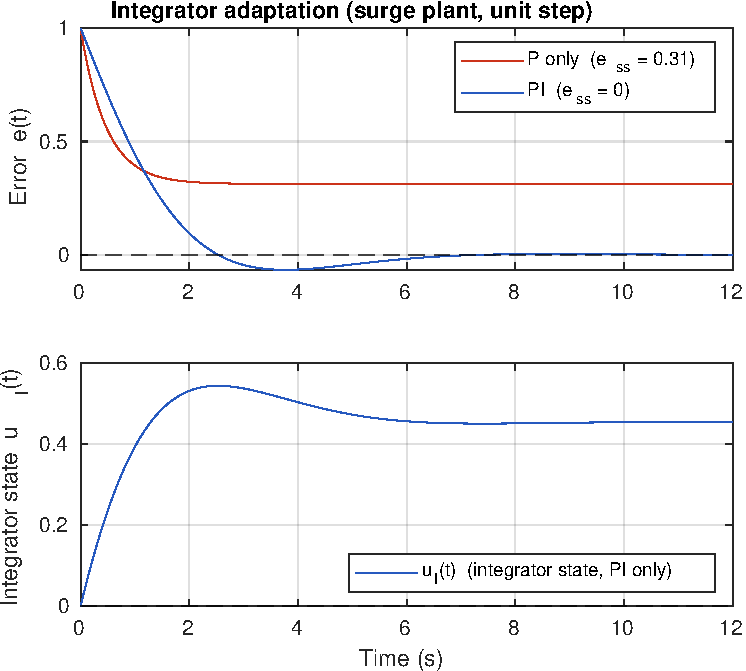
\includegraphics[width=0.75\linewidth]{images/sse_integrator_adapt.pdf}
\caption{Integrator adaptation for a unit step command on the surge plant
  ($K = 2.2$, $\tau = 1.5$\,s).
  \emph{Top:} tracking error $e(t)$.  P-only settles to a permanent offset;
  PI drives $e \to 0$.
  \emph{Bottom:} integrator state $u_I(t) = K_I\!\int_0^t\! e\,d\tau$
  (PI controller only).  The integrator charges up while
  $e > 0$, providing a persistent bias to the plant.  Once $e \approx 0$,
  the integrator holds constant --- encoding the steady-state throttle needed
  to maintain the commanded speed despite the plant's finite DC gain.}
\label{fig:integrator_adapt}
\end{figure}

\subsection{The Trade-offs}

Integral action is not free.  The costs (discussed at length in the PID article)
bear repeating here in the context of steady-state error:

\begin{description}
  \item[Slower settling or more overshoot.]  Adding an integrator raises
    the closed-loop order.  A first-order plant with P control gives a
    first-order closed loop; with PI it becomes second-order and can
    oscillate.  The gain $K_I$ must be chosen carefully.
  \item[Integral windup.]  When the actuator saturates, the plant no longer
    follows the controller.  The integrator keeps charging, accumulating a
    large bias; when saturation clears, that bias drives overshoot.
    Anti-windup is required in any real implementation.
  \item[Harder to stabilize.]  Every integrator makes the system harder to keep
    stable --- we will return to this in the frequency response article.
\end{description}

% ===========================================================================
\section{Integrator vs.\ Feedforward: Practical Trade-offs}
\label{sec:ff_vs_int}
% ===========================================================================

There are two fundamentally different strategies for reducing steady-state
error.  The PID article introduced both; we now compare them directly in
the framework of steady-state error analysis.

\subsection{Feedforward Does Not Change System Type}

A feedforward path injects the reference $R(s)$ directly into the plant
command, bypassing the error signal.  \Cref{fig:ff_structure} shows the
architecture: the gain $1/K$ (the inverse of the plant's DC gain) routes
the reference directly to the plant input, providing the known steady-state
effort immediately.

\begin{figure}[htbp]
\centering
\begin{tikzpicture}[
  >=Latex, thick,
  block/.style = {draw, rectangle, minimum height=2.5em, minimum width=4.5em},
  sum/.style   = {draw, circle, inner sep=0pt, minimum size=1.2em},
]
  \node[coordinate]                    (rin)   {};
  \node[sum,   right=1.4cm of rin]     (esum)  {};
  \node[block, right=1.8cm of esum]    (C)     {$C(s)$};
  \node[sum,   right=1.8cm of C]       (usum)  {};
  \node[block, right=1.8cm of usum]    (P)     {$P(s)$};
  \node[coordinate, right=1.4cm of P]  (yout)  {};

  \node[block, above=1.0cm of usum, minimum width=5em] (FF) {$1/K$};

  \node[font=\scriptsize, inner sep=0pt, anchor=south east] at (esum.north west) {$+$};
  \node[font=\scriptsize, inner sep=0pt, anchor=north east] at (esum.south west) {$-$};
  \node[font=\scriptsize, inner sep=0pt, anchor=north east] at (usum.south west) {$+$};
  \node[font=\scriptsize, inner sep=0pt, anchor=south east] at (usum.north west) {$+$};

  \coordinate (rbranch) at ($(rin)!0.6!(esum)$);
  \fill (rbranch) circle (2pt);
  \draw[->] (rin)     -- node[above]{$R(s)$} (esum);
  \draw[->] (rbranch) |- (FF);
  \draw[->] (FF)      -- (usum.north);
  \draw[->] (esum)    -- node[above]{$E(s)$} (C);
  \draw[->] (C)       -- (usum);
  \draw[->] (usum)    -- node[above]{$U(s)$} (P);
  \draw[->] (P)       -- node[above]{$Y(s)$} (yout);

  \coordinate (fbk) at ($(P.east)!0.5!(yout)$);
  \draw[->] (fbk) -- ++(0,-1.8) -| (esum.south);
\end{tikzpicture}
\caption{Proportional controller with feedforward gain $1/K$.  The reference
  drives two paths: the standard error-based feedback path, and a direct path
  to the plant input that supplies the steady-state effort without waiting for
  error to accumulate.}
\label{fig:ff_structure}
\end{figure}

At steady state, the feedforward injects $r/K$ directly.  Since the plant's
DC gain is $K$, the output becomes $K \cdot r/K = r$ --- tracking is exact.
But this relies on knowing $K$ precisely.  If the actual plant gain differs
from the model (e.g., due to loading, temperature, or aging), a residual
error remains.

More importantly for our analysis: \textbf{the feedforward path does not
change the open-loop transfer function $G(s)$}.  System type is unchanged.
The standard error formula \cref{eq:ess_general} does not capture feedforward
because the formula models the feedback loop in isolation.  The feedforward
result is not in contradiction --- it just requires a separate accounting.

\subsection{Side-by-Side Comparison}

\begin{table}[htbp]
\centering
\caption{Integrator vs.\ feedforward for eliminating steady-state error.}
\label{tab:int_vs_ff}
\begin{tabular}{p{2.4cm}p{5.0cm}p{5.0cm}}
\toprule
 & \textbf{Integral action} & \textbf{Feedforward} \\
\midrule
Mechanism
  & Accumulates error until $e = 0$; model-free.
  & Directly commands the steady-state effort; model-dependent. \\[4pt]
Model knowledge
  & None required; works despite gain drift or calibration error.
  & Requires accurate plant DC gain $K$; errors leave a residual offset. \\[4pt]
Transient response
  & Slower settling; possible overshoot; windup during saturation.
  & Fast settling; shape nearly identical to proportional-only response. \\[4pt]
System type
  & Increments by 1; captured by \cref{eq:ess_general}.
  & No change; feedforward is outside the formula's scope. \\[4pt]
Disturbance rejection
  & Yes --- integrator responds to any persistent mismatch, including loads and currents.
  & No --- feedforward acts only on the reference, not unmeasured disturbances. \\[4pt]
\bottomrule
\end{tabular}
\end{table}

\subsection{The Combined Approach: PI with Feedforward}

In practice the two strategies complement each other.  Feedforward provides
fast, low-overshoot response; the integrator provides robustness to model
uncertainty and disturbances.  \Cref{fig:ff_compare} compares four
architectures on the surge plant.

\begin{figure}[htbp]
\centering
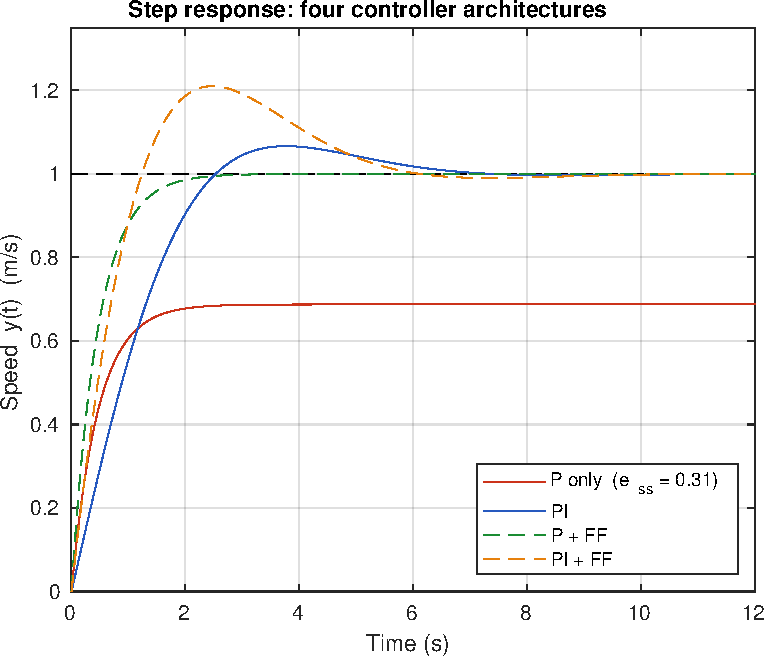
\includegraphics[width=0.75\linewidth]{images/sse_ff_compare.pdf}
\caption{Step responses for four controller architectures on the surge plant
  ($K = 2.2$, $\tau = 1.5$\,s).
  \textbf{P only:} fast but settles below the setpoint (Type~0, finite error).
  \textbf{PI:} zero steady-state error but slower with mild overshoot.
  \textbf{P\,+\,FF:} zero error \emph{and} fast settling, but would leave a
  residual offset if the plant gain were mis-estimated.
  \textbf{PI\,+\,FF:} zero error, fast settling, and robust to model error ---
  the preferred combination for step tracking on a modeled plant.}
\label{fig:ff_compare}
\end{figure}

The PI\,+\,feedforward combination is often the first choice when a plant model
is available.  The feedforward handles the bulk of the effort immediately;
the integrator corrects whatever residual error remains due to disturbances or
model mismatch.  Together they provide what neither alone achieves: speed
\emph{and} robustness.

The script \texttt{sse\_companion.m} (same directory as this article) generates
all figures and demonstrates the numerical computations shown here.

\end{document}
